\documentclass{article}
\usepackage[utf8]{inputenc}
\usepackage{amsmath}
\usepackage{amsthm}
\usepackage{amssymb}
\usepackage{natbib}
\usepackage{dsfont}
\usepackage{stmaryrd}
\usepackage{geometry}
\usepackage{graphicx}
\usepackage[T1]{fontenc}
\usepackage{listings}
\usepackage[french, ruled, vlined]{algorithm2e}
\renewcommand{\abstractname}{Résumé}
\geometry{vmargin=2cm}
\usepackage{subfig}
\usepackage{color}
\begin{document}
\title{Pricing d'options par FFT}
\author{LE FAY Yvann, GOUMENT Daniel, DE LAHARPE Gabriel}
\date{Janvier 2022}
\maketitle
\begin{center}
	\includegraphics[height=2in]{/home/grothendieck/1A/ENSAE1A/info/LOGO-ENSAE.png}
\end{center}
\begin{abstract}
	Nous proposons une méthode de pricing d'options européennes dont l'on connaît la fonction caractéristique $\varphi$ de $\log S_t$ en utilisant la formule d'inversion de Carr-Madan. Cette formule donne la solution analytique du prix de l'option sous la forme d'une transformée de Fourier, ce qui permet, grâce à la transformée de Fourier discrète, de calculer une solution approchée en complexité $O(N\log N)$. 

	Nous nous referons à la thèse de master de ManWo Ng, PhD, "Option Pricing via the FFT".
\end{abstract}

\section{Modèles de pricing}
\subsection{Modèle de Black-Scholes}

Le prix du sous-jacent $S_t$ ($s_t = \log S_t$) suit un mouvement brownien géométrique, ici $W_t\sim \mathcal{N}(0, t)$, 
\begin{align*}
	\mathrm{d}S_t = rS_t\mathrm{d}t + \sigma S_t \mathrm{d}W_t
\end{align*}

Ce qui se résout sous forme close en
\begin{align*}
	S_t = S_0\exp\big\{(r-\sigma^2/2)t+\sigma W_t\big\}
\end{align*}

La fonction caractéristique est 
\begin{align*}
	\varphi(u) = \exp\big\{iu(s_0+(\mu-\sigma^2/2)t)-1/2u^2\sigma^2t)\big\}
\end{align*}
\subsection{Modèle de Merton}
Le prix du sous-jacent suit un mouvement brownien géométrique auquel on rajoute un processus de Poisson $Z_t$ avec une distribution log-normale des tailles de jumps $Y_i\sim \mathcal{N}(\mu, \delta^2)$ indépendants de $W_t$ et de $N_t$ le processus de Poisson d'intensité $\lambda$ indépendant de $W_t$ que suivent les jumps. Merton propose

\begin{align*}
	\frac{\mathrm{d}S_t}{S_t} = r\mathrm{d}t + \sigma\mathrm{d}W_t + \mathrm{d}Z_t
\end{align*}

Ce qui se résout en
\begin{align*}
	S_t = S_0 \exp\big\{\mu^M t +  \sigma W_t + \sum_{i=1}^{N_t} Y_i\big\}
\end{align*}

où $\mu^M = r - \sigma^2-\lambda\{\exp(\mu+\delta^2/2)-1\}$. 

La fonction caractéristique est
\begin{align*}
	\varphi(u) = \exp\{t(-\sigma^2u^2/2+i\mu^M u + \lambda(e^{-\delta^2u^2/2+i\mu u -1}))+is_0\}
\end{align*}

\subsection{Modèle de Heston}
Nous précisons pas ici le modèle, voir Hull et White (1987) pour plus de détails. La fonction caractéristique est
\begin{align*}
	\varphi(u)e^{-ius_0} = \frac{\exp\{\kappa \theta t(\kappa - i \rho v u)/v^2+iut r\}}{(\cosh\frac{\gamma t}{2}+\frac{\kappa-i\rho v u }{\gamma}\sinh\frac{\gamma t }{2})^{\frac{2\kappa \theta}{v^2}}}\exp\{-\frac{(u^2+iu)v_0}{\gamma \coth\frac{\gamma t}{2}+\kappa-i\rho v u}\}
\end{align*}
où $\gamma(u) = \sqrt{v^2(u^2+iu)+(\kappa-i\rho v u)^2}$

\section{Pricing avec FFT}
\subsection{Formule d'inversion de Carr-Madan}
Notons $S_T$ le price à la maturité du sous-jacent pour un call européen de strike $K$. Définissons $s_T = \log S_T$ et la densité risque-neutre $q_T$. La fonction caractéristique de $q_T$ est
\begin{align*}
	\varphi_T(u) = \int_{\mathbb{R}}e^{ius}q_T(s)\mathrm{d}s
\end{align*}

Posons $k = \log K$, la principe de valorisation risque-neutre donne le prix du call
\begin{align*}
	C_T(K) &= e^{-rT}\mathbb{E}(S_T-K)^+\\
	&= e^{-rT}\int_{k}^{\infty}(e^s-e^k)q_T(s)\mathrm{d}s
\end{align*}

avec $\lim_{K\to 0} C_T(K)= S_0$. On voit donc que $k \mapsto C_T(e^k)$ n'est pas dans $L^1$. Ainsi l'intégrale de Fourier n'existe pas. Considérons une version modifiée du prix, soit $\alpha >0$ que l'on viendra préciser plus tard,  
\begin{align*}
	c_T(k) = e^{\alpha k}C_T(e^k)
\end{align*}
avec $\alpha$ tel que $c_T$ admet une transformée de Fourier. Notons $\psi_T$ la transformée de Fourier de $c_T$, 
\begin{align*}
	\psi_T(u) = \int_{\mathbb{R}}e^{iuk}c_T(k)\mathrm{d}k
\end{align*}

La transformée de Fourier inverse donne
\begin{align*}
	C_T(K) = \frac{e^{-\alpha k}}{2\pi}\int_{\mathbb{R}}e^{-i u k} \psi_T(u)\mathrm{d}u = \frac{e^{-\alpha k}}{\pi}\textup{Re}\bigg\{\int_{0}^{\infty}e^{-i u k}\psi_T(u)\mathrm{d}u\bigg\}
\end{align*}

A l'aide de Fubini, on obtient
\begin{align*}
\psi_T(u) = \frac{e^{-rT}\varphi_T(u-(\alpha+1)i)}{\alpha^2+\alpha-u^2+i(2\alpha+1)u)}
\end{align*}

Une condition suffisante pour que $c_T \in L^1$, est $\mathbb{E}S_T^{\alpha+1} < \infty$.
\subsection{Approximation numérique et FFT}
Il s'agit d'approcher $C_T$ par 
\begin{align*}
	\frac{\exp(-\alpha k)}{\pi}\textup{Re}\bigg\{\sum_{j=0}^{N-1} e^{-i \eta j k}\psi(\eta j)\eta\bigg\}
\end{align*}

La somme dans la partie réelle se calcule à l'aide d'un algorithme FFT. L'algorithme de Turkey-Cooley permet de calculer les sommes de la forme $\sum_{j=0}^{N-1} e^{-i\frac{2\pi}{N} j u} x_j$ pour $u=0,\ldots, N-1$ en un temps $O(N\log N)$ en suivant un principe de "diviser pour mieux régner".

On considère des log-strikes réparties uniformément près du log-prix $s_0$, 
\begin{align*}
	k_u = s_0 + \zeta u - \frac{1}{2}N\zeta
\end{align*}
pour $u = 0, \ldots, N-1$.

On obtient
\begin{align*}
	C_T(k_u) \approx \frac{\exp(-\alpha k_u)}{\pi} \textup{Re}\bigg\{\sum_{j=0}^{N-1}e^{-i\zeta \eta j u} e^{i\{(\frac{1}{2}N\zeta-s_0)\eta j\}}\psi(\eta j)\eta\bigg\}
\end{align*}

Il s'agit donc d'appliquer l'algorithme FFT sur les $x_j= e^{i\{(\frac{1}{2}N\zeta-s_0)\eta j\}}\psi(\eta j)$ pour $j=0,\ldots, N-1$, en fixant la condition \begin{align*}
	\zeta \eta = \frac{2\pi}{N}
\end{align*}

Le paramètre $N$ caractérise le temps de calcul, la variable $\zeta$ caractérise le pas pour les log-strikes. On souhaite $\zeta$ aussi petit que possible de manière à avoir le plus de points proches de $s_0$, où l'approximation est la meilleure. Mais la contrainte précédente impose alors un paramètre $\eta$ plus grand, ce qui vient diminuer la qualité d'approximation de l'intégrale de Fourier par la Fourier discrète.

\subsection{Choix de $\alpha$}
Il est montré dans "Option Pricing via the FFT" que la valeur $\alpha = 0.75$ (celle choisie dans le programme) est telle que $\mathbb{E}S_T^{1+\alpha} <\infty$ pour les modèles ici considérés, ce qui permet l'application de la transformation de Carr-Madar. Toutefois, le choix de $\alpha$ impacte la tractabilité du calcul de l'intégrale de Fourier car celle-ci vient modifier les oscillations de l'intégrande. 

Il est convenable de penser qu'une valeur $\alpha$, fonction des paramètres du modèle, qui minimise l'intégrande, rende le calcul plus tractable, 
\begin{align*}
	\alpha = \textup{argmin}_{\alpha > 0} \textup{sup}_{u\in\mathbb{R}}\big\|\frac{e^{-rT}\phi_T(u-(\alpha+1)i)}{\alpha^2+\alpha-u^2+i(2\alpha+1)u}\big\|
\end{align*}

Voir la référence pour des expressions analytiques dans les cas de Black-Scholes et Heston de $\alpha$.
\subsection{Structure, utilisation du programme et difficultés rencontrées}
Dans ce projet, nous avons fait le choix d’organiser notre code autour de l’utilisation de classes. Ceci nous a permis de profiter des avantages offerts par la programmation orientée objet.

\begin{itemize}
	\item La classe \lstinline{ClosedForm} permet le calcul des prix à partir de la formule close dans le modèle de Black Scholes pour un call européen. Elle contient les attributs suivants : risk free rate, volatilité, maturité et prix $S$ du sous-jacent en 0.
	\item La classe \lstinline{fft} permet de calculer la FFT d’un tableau en $O(N\log N)$.
	\item La classe \lstinline{Cdf} (respectivement \lstinline{CdfMerton} et \lstinline{CdfHeston}) permet de calculer la fonction de répartition du log du prix du sous jacent ainsi que la transformée de Fourier de $c_T$ pour le modèle de Black Scholes (respectivement Black Scholes Merton et Heston).
	\item La classe \lstinline{Calculator} (respectivement \lstinline{CalculatorMerton}, \lstinline{CalculatorHeston}) permet de calculer la liste des prix de call pour une liste de strikes autour du prix du sous jacent en 0 en suivant le modèle de Black Scholes (respectivement Black Scholes, Merton, Heston).
\end{itemize}
L’utilisation du fichier main.cpp se décompose en cinq parties :
\begin{itemize}
	\item Remplissage des paramètres propres au modèle que l’on souhaite utiliser (dans le code donné en exemple, tous les modèles sont utilisés)
        \item Construction d’un objet de la classe de calcul correspondant au modèle utilisée : \lstinline{ClosedForm} pour un calcul de call européen à l’aide de la formule exacte et \lstinline{Calculator} (respectivement \lstinline{CalculatorMerton}, \lstinline{CalculatorHeston} pour les modèles de Black Scholes, BSMerton ou Heston) à l'aide de la méthode FFT.
	\item Construction d’une liste qui va contenir les strikes (ou les log-strikes dans le cas des calculator FFT) et d’une liste qui va contenir les valeurs des call correspondants.
	\item Appel de la fonction de calcul de la classe correspondante (utilisation d’une boucle for pour la closed form).
	\item Extraction des résultats à l’aide de la fonction correspondante (ClosedForm ou FFT) dans un fichier texte. Ici, les résultats sont dans un format adapté à la lecture par Mathematica. Les fonctions d’extraction peuvent être modifiées afin que les résultats sortent dans un format lisible par Pandas par exemple.
\end{itemize}

Chaque membre du groupe a déjà une certaine expérience en programmation et a déjà fait de la POO. Nous n'avons donc rencontré aucune véritable difficulté.

L'étape majeure du projet a été de penser la structure du programme : établir les classes, puis les fonctions et les variables que chacune avaient en commun de manière à bien exploiter l'héritage.
O
Ce projet a été pour nous l'occasion de se familiariser avec la syntaxe C++, quelques techniques en calcul numérique (algorithme FFT), ainsi que sur différents modèles de pricing.
\subsection{Comparaisons numériques}
On pose, $N = 8192$, $r = 0.05$, $v = 0.7$, $\sigma=0.2$, $T=1$, $S_0 = 100$, $\eta = 0.0125$, $\alpha = 0.75$, $\rho = -0.5$, $v_0 = 0.2$, $\lambda = 0.13$, $\mu = 0$, $\delta = 0.0004$, $\kappa = 10$.

On compare les résultats obtenus par FFT avec, lorsque l'on peut, les résultats obtenus avec la forme close. Dans le cas où l'on ne connaît pas la forme close, on compare les résultats FFT avec ceux obtenus par la méthode $\textup{NIntegrate}$ de Mathematica pour l'évaluation de l'intégrale de Fourier définissant $C_T$. Voir Fig. 1, 2 et 3.

\begin{figure}[h]
	\centering
	\subfloat{{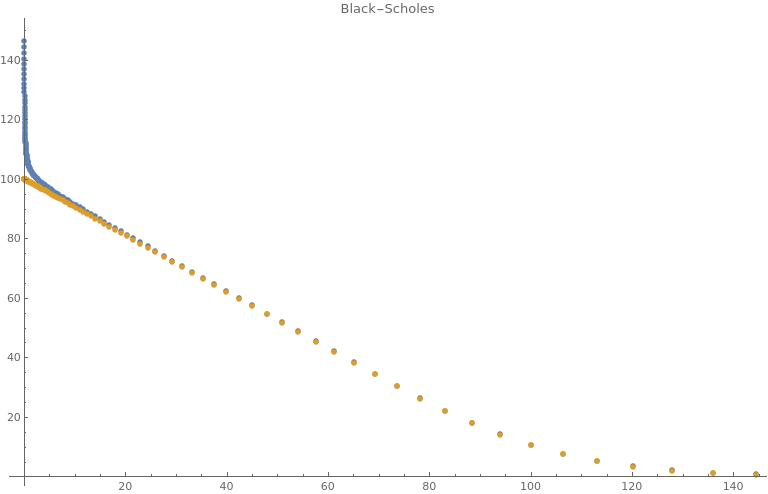
\includegraphics[scale=0.25]{/home/grothendieck/BS0.jpg}}}
	\qquad
	\subfloat{{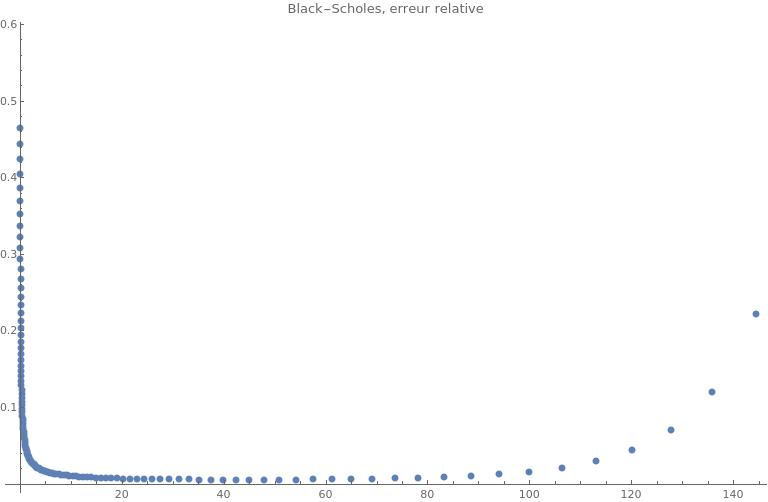
\includegraphics[scale=0.25]{/home/grothendieck/BS1.jpeg}}}
	\caption{A gauche, en bleu FFT, en orange forme close}
	\subfloat{{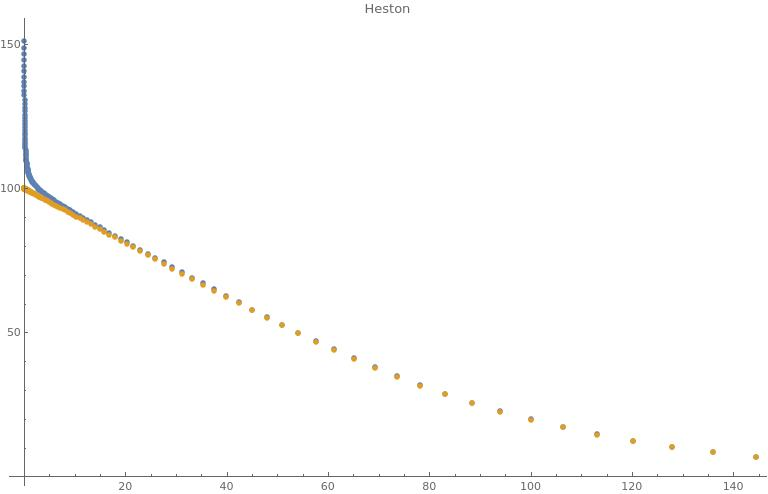
\includegraphics[scale=0.25]{/home/grothendieck/Heston0.jpg}}}
	\qquad
	\subfloat{{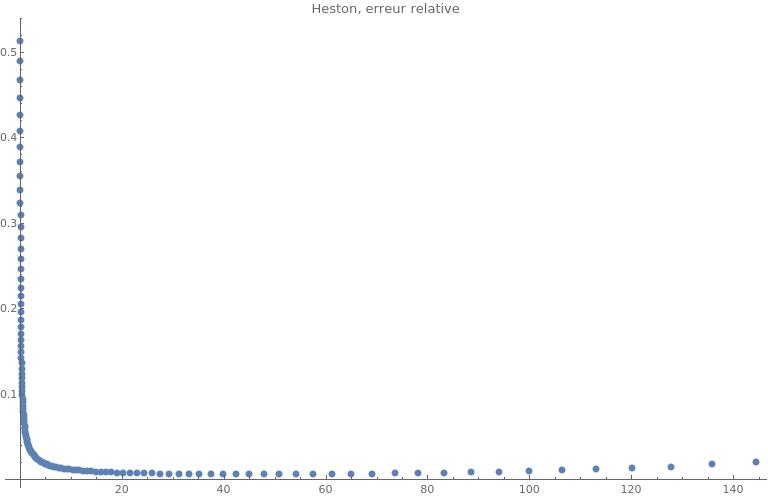
\includegraphics[scale=0.25]{/home/grothendieck/Heston1.jpeg}}}
	\caption{A gauche en orange, NIntegrate de Mathematica}
	\subfloat{{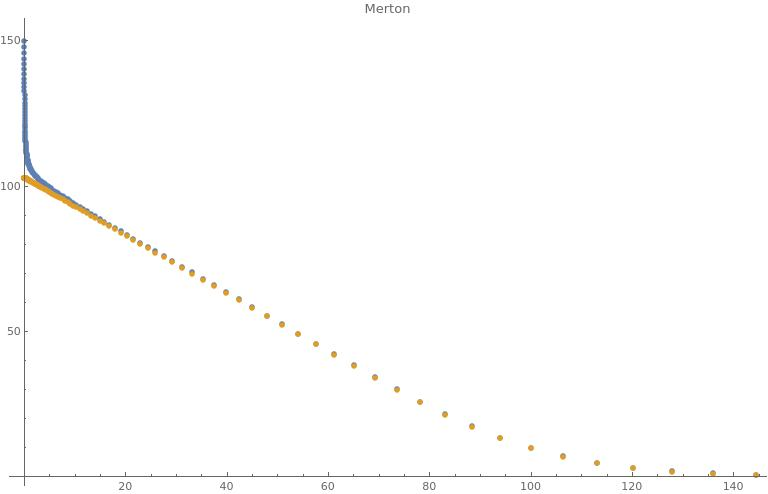
\includegraphics[scale=0.25]{/home/grothendieck/Merton0.jpg}}}
	\qquad
	\subfloat{{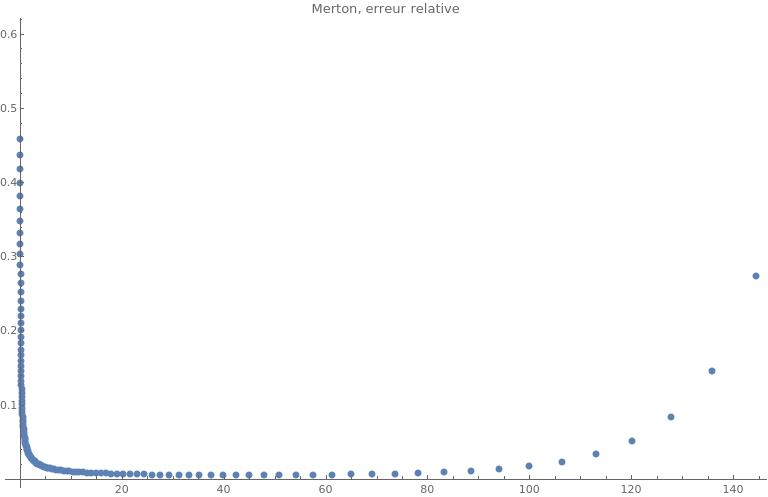
\includegraphics[scale=0.25]{/home/grothendieck/Merton1.jpg}}}
	\caption{A gauche en orange, NIntegrate de Mathematica}
\end{figure}
\subsection{Comparaison avec Monte-Carlo}
Il est difficile d'effectuer une comparaison toutes choses égales par ailleurs de l'algorithme présenté avec celui de Monte-Carlo. L'algorithme de MC a une complexité qui dépend de la précision attendue entre le prix Monte-Carlo et le prix exact. En effet, si on fait $M$ tirages, le théorème centrale limite assure que la différence est de l'ordre de $1/\sqrt{M}$. Ainsi, à une précision $\varepsilon$ fixée, la complexité de l'algorithme est $O(M) = O(1/\varepsilon^2)$. Cet algorithme donne le prix pour une seule valeur de strike. 

Dans le cas de l'algorithme FFT, le paramètre qui caractérise la complexité est $N$, le nombre de valeurs de strike. L'écart entre l'intégrale exacte de Fourier et la transformée de Fourier discrète n'est pas explicite (à notre connaissance) mais dépend positivement de $\eta$ i.e négativement de $N$.

Ainsi, on contrôle la précision dans un premier cas mais pas dans le second, dans le premier cas on calcule $C_T$ pour un strike, dans le second pour $N$. La comparaison est délicate. 

Toutefois, il est possible de trouver une configuration des deux méthodes de manière à obtenir des valeurs numériques similaires. Alors dans ce cas, il est possible de comparer le temps de calcul des deux algorithmes. Voir le tableau suivant.
\begin{figure}
	\centering
\begin{tabular}{lll}
	Modèle & FFT & MC\\
	\hline
	Merton & 0.01 & 25.1\\
	Heston & 0.01 & 27.6\\
\end{tabular}
\caption{Temps de calcul en secondes pour les deux méthodes, 20 strikes différents et résultats moyennés sur 5000 essais.}
\end{figure}
\end{document}

